\documentclass[11pt]{article}

\usepackage[a4paper,margin=1in]{geometry}
\usepackage{graphicx}
\usepackage{booktabs}
\usepackage{array}
\usepackage{longtable}
\usepackage{amsmath,amssymb}
\usepackage{hyperref}
\usepackage{fancyhdr}
\usepackage{titlesec}
\usepackage{xcolor}
\usepackage{enumitem}
\usepackage{caption}
\usepackage{tikz}
\usetikzlibrary{shapes.geometric,arrows.meta,positioning,fit}
\tikzset{
  pbox/.style={rectangle, rounded corners, draw=kuetblue, fill=kuetblue!12, text width=2.6cm, minimum height=1.3cm, align=center, font=\small, inner sep=4pt},
  pboxend/.style={pbox, fill=green!18, draw=green!45!black},
  pboxwarn/.style={pbox, fill=red!12, draw=red!60!black},
  parrow/.style={-{Stealth[length=2.5mm]}, thick, kuetblue}
}

\definecolor{kuetblue}{RGB}{31,73,125}
\hypersetup{colorlinks=true, linkcolor=kuetblue, citecolor=kuetblue, urlcolor=kuetblue}

\pagestyle{fancy}
\fancyhf{}
\fancyhead[L]{Machine Learning Laboratory - CSE 4112}
\fancyhead[R]{KUET}
\fancyfoot[C]{\thepage}
\renewcommand{\headrulewidth}{0.4pt}

\titleformat{\section}{\Large\bfseries\color{kuetblue}}{\thesection.}{0.5em}{}
\titleformat{\subsection}{\large\bfseries\color{kuetblue}}{\thesubsection}{0.5em}{}

\newcolumntype{L}[1]{>{\raggedright\arraybackslash}p{#1}}

\title{
\vspace{-1cm}

\includegraphics[width=2.3cm]{figures/kuet_logo.png}\\[0.3cm]
\textbf{\color{kuetblue}\Large KHULNA UNIVERSITY OF ENGINEERING \& TECHNOLOGY}\\[0.2cm]
\large Department of Computer Science and Engineering\\[0.5cm]
\textbf{\Large Machine Learning Laboratory}\\
\textbf{Course Code: CSE 4112}\\[0.5cm]
\textbf{\Large Project Report}\\[0.3cm]
{\color{kuetblue}\Large\textbf{Occlusion-Robust Face Identification Using a\\ Pretrained ArcFace Model}}\\[0.3cm]
\large Submission Date: 08/09/2026
}
\author{}
\date{}

\begin{document}
\begin{titlepage}
\maketitle
\thispagestyle{empty}
\vspace{1cm}
\begin{minipage}[t]{0.48\textwidth}
\textbf{Submitted to,}\\[0.3cm]
\textbf{Dr. Muhammad Aminul Haque Akhand}\\
Professor\\
Department of Computer Science and Engineering\\[0.4cm]
\textbf{Nabil Faiyaz Sadi}\\
Lecturer\\
Department of Computer Science and Engineering
\end{minipage}
\hfill
\begin{minipage}[t]{0.48\textwidth}
\textbf{Submitted by,}\\[0.3cm]
Roll: 2107031, 2107044, 2107046,\\
2107047, 2107057, 2107059\\[0.4cm]
Section: A\\
Year: 4th\\
Semester: 1st
\end{minipage}
\vfill
\begin{center}
Khulna-9203, Bangladesh
\end{center}
\end{titlepage}

\tableofcontents
\newpage

\section{Introduction}

Modern face-recognition systems perform well when a frontal face is clear, well illuminated, and similar to the images used during training. Their performance can fall sharply when identity-bearing facial regions are hidden by a medical mask, sunglasses, a scarf, a cap, or a combination of these, or when lighting and head pose change. This project addresses the problem as \textbf{closed-set face identification}: every test image is assumed to belong to a person already enrolled, and the system returns the corresponding participant ID (e.g.\ \texttt{p07}) rather than merely detecting whether an occlusion is present.

The final system is a consent-based local dataset of 30 enrolled participants, captured under eight covering conditions and two lighting levels, processed through a fixed detect-align-crop pipeline, and classified with a \textbf{pretrained ArcFace (iResNet50) embedding model} paired with a \textbf{RetinaFace} detector. Three experiments were run to determine how much task-specific training improves a pretrained face embedding, and specifically whether occlusion-diverse training data is necessary for that improvement to hold under compound occlusions. The completed system was packaged into a phone-camera live demonstration served from a laptop over the local network.

This report documents what was actually collected and built, compares the approach against closely related published work, and reports the deviations from the original proposal.

\section{Problem Statement and Objectives}

\subsection{Problem Statement}

Given an input image containing a normal or partially occluded face, the system must classify the image as one of 30 enrolled identities. Different occlusions hide different facial regions: a mask removes the nose, mouth, and jawline; sunglasses remove much of the eye region; a cap changes the forehead and hairline; low light reduces visible texture generally. The central question is whether a pretrained face-embedding model, given only a small amount of per-identity data (a few hundred images per person across all conditions combined), can produce identity features that stay discriminative under these conditions without being explicitly retrained on masks or sunglasses from scratch.

\subsection{Objectives and Completion Status}

\begin{enumerate}[label=\arabic*.]
\item Collect a structured face-image dataset covering a range of occlusion and lighting conditions. \textbf{Completed} — 30 participants, 6{,}000 raw images.
\item Capture each participant under eight covering conditions: none, cap, mask, sunglasses, scarf, clear glasses, mask+sunglasses, mask+clear glasses. \textbf{Completed.}
\item Detect, align, crop, resize, and quality-check every face image using one reproducible preprocessing pipeline. \textbf{Completed} — 5{,}988/6{,}000 images (99.8\%) successfully detected and aligned.
\item Split the dataset into train/validation/test sets such that every identity, and where possible every identity--occlusion combination, appears in all three splits. \textbf{Completed.}
\item Evaluate a pretrained ArcFace pipeline with two forms of task-specific training: a trained classification head, and partial backbone fine-tuning. \textbf{Completed} — three experiments, E1--E3.
\item Evaluate overall accuracy, per-participant accuracy, and per-occlusion accuracy. \textbf{Completed} — extended beyond the original plan to also include per-occlusion precision/recall/F1 and a full $30\times30$ confusion matrix for every experiment (Section~\ref{sec:results}).
\item Produce a working demonstration that predicts the enrolled participant from a live phone camera. \textbf{Completed} — a browser-based demo streamed from a phone to a laptop over HTTPS on the local network.
\end{enumerate}

\section{Related / Base Papers}
\label{sec:related}

This project builds on three published works, chosen to cover the two halves of the problem separately: one supplies a dataset/capture precedent, and two supply recognition-method precedents. Table~\ref{tab:base-papers} summarises each and how it is used here; the detailed three-way comparison against this project's own results is given later in Table~\ref{tab:comparison}.

\begin{table}[h]
\centering
\caption{Base papers used for comparison.}
\label{tab:base-papers}
\begin{tabular}{L{3.3cm}L{5.3cm}L{5.7cm}}
\toprule
\textbf{Paper} & \textbf{Main contribution} & \textbf{Relation to this project} \\
\midrule
Salari and Rostami, ``Pgu-Face: A Dataset of Partially Covered Facial Images,'' \emph{Data in Brief}, 2016 \cite{pguface2016} &
Introduces the Pgu-Face dataset: 896 images from 224 subjects, four images per subject, across up to two sessions at least six days apart, under clean-shaven/stubble conditions with and without sunglasses. Does not propose a recognition model. &
Closest public dataset precedent for identity-labelled, partially-covered face capture with a controlled protocol; this project's dataset (6{,}000 images, 30 identities, 8 occlusion types) is far larger in image count and occlusion variety, though over far fewer identities and (unlike Pgu-Face) a single session. \\[0.4cm]
Chong, Chong, and Ong, ``Masked Face Recognition Using Support Vector Machine and Convolutional Neural Network,'' \emph{ICoICT}, 2022 \cite{chong2022svm} &
Trains a CNN for feature extraction and an SVM for label classification on masked-face benchmarks (RMFD, LFW-SMFD); reports 98.39\% TAR on a 50-category RMFD subset, with a marked accuracy drop as the category count grows, since SVM classification does not scale well to more identities. &
Closest published recognition-method precedent using a trained classifier on top of extracted features; this project instead adapts a pretrained ArcFace embedding rather than training a CNN feature extractor from scratch, and trains a lightweight identity head instead of an SVM. \\[0.4cm]
Montero, Nieto, Leskovsky, and Aginako, ``Boosting Masked Face Recognition with Multi-Task ArcFace,'' \emph{SITIS}, 2022 \cite{montero2022mtarcface} &
Extends an ArcFace-based ResNet50 pipeline with masked-face training augmentation and an auxiliary mask-detection output, so the same network both recognises identity and predicts whether a mask is present. &
Directly comparable ArcFace-family model adapted specifically for masks at larger scale; shows what mask-specific architecture changes buy over the untouched pretrained embedding this project starts from, and is the closest precedent for treating occlusion-diverse training data as the key lever, matching this project's own E1-vs-E2 finding (Section~\ref{sec:results}). \\
\bottomrule
\end{tabular}
\end{table}

\section{Dataset}
\label{sec:dataset}

\subsection{Team and Participants}

Thirty identities (\texttt{p01}--\texttt{p30}) were enrolled, contributed by six team members who each recruited and photographed five people (themselves plus four relatives/acquaintances who gave consent). The full participant-to-photographer mapping is kept in \texttt{metadata/person\_id\_mapping.txt} and is not reproduced here since it is an internal bookkeeping file, not a reportable result.

\subsection{Consent}

Every participant signed a consent form before any photograph was taken. The form explains that this is an academic, non-commercial prototype; that each participant is assigned an anonymous ID (e.g.\ \texttt{p07}) and never labelled by name; that raw images and the identity mapping are restricted to the six project members and never published outside the group; that participation is voluntary and withdrawable; and that a recognisable photo is only shown in the report, presentation, or demonstration for participants who separately tick an optional permission box.

\subsection{Capture Protocol}

Each participant was photographed under eight covering conditions --- \texttt{none}, \texttt{cap}, \texttt{mask}, \texttt{scarf}, \texttt{clearglass}, \texttt{sunglass}, \texttt{mask\_clearglass}, \texttt{mask\_sunglass} --- crossed with two lighting levels, \texttt{regular} and \texttt{low}. Collection happened in a single sitting per participant, with participants naturally varying their head position across shots rather than posing to a separately-logged pose label. The realised dataset totals \textbf{6{,}000 images}: 30 identities $\times$ 200 images (25 images per occlusion/lighting cell on average), which comfortably exceeds the proposal's original target of 10--15 participants.

Filenames follow a fixed pattern, e.g.\ \texttt{p07\_mask\_sunglass\_low\_014.jpg}, so identity, occlusion, and lighting can be parsed without a lookup table; a manifest CSV remains the authoritative metadata source.

\subsection{Pose, Lighting, and Obstruction Categories}
\label{sec:categories}

Table~\ref{tab:pose-labels} records the head-pose variation participants were asked to move through informally during capture (not logged as a separate per-image field); Table~\ref{tab:lighting-labels} and Table~\ref{tab:obstruction-labels} record the two dimensions that \emph{are} logged for every image, since occlusion and lighting are what this project's identification task is actually evaluated against.

\begin{table}[h]
\centering
\caption{Head-pose variation encouraged during capture.}
\label{tab:pose-labels}
\begin{tabular}{L{3cm}L{9cm}}
\toprule
\textbf{Label} & \textbf{Meaning} \\
\midrule
front & Looking directly at the camera. \\
left / right & Head turned to the participant's left / right. \\
up / down & Chin tilted upward / downward. \\
\bottomrule
\end{tabular}
\end{table}

\begin{table}[h]
\centering
\caption{Lighting labels used during capture.}
\label{tab:lighting-labels}
\begin{tabular}{L{3cm}L{9cm}}
\toprule
\textbf{Label} & \textbf{Meaning} \\
\midrule
regular & Even indoor lighting; the face is clearly visible. \\
low & Dim lighting; the face is dimmer but still detectable. \\
\bottomrule
\end{tabular}
\end{table}

\begin{table}[h]
\centering
\caption{Obstruction (covering) labels used during capture.}
\label{tab:obstruction-labels}
\begin{tabular}{L{3cm}L{9cm}}
\toprule
\textbf{Type} & \textbf{Labels} \\
\midrule
Single covering & \texttt{none}, \texttt{mask}, \texttt{sunglass}, \texttt{clearglass}, \texttt{scarf}, \texttt{cap} \\
Combined covering & \texttt{mask\_sunglass}, \texttt{mask\_clearglass} \\
\bottomrule
\end{tabular}
\end{table}

Figure~\ref{fig:sample-accepted} shows one accepted example per occlusion family, and Figure~\ref{fig:occ-counts} gives the exact image count preprocessing produced for each of the eight conditions -- close to, but not perfectly, balanced, since a small number of images per condition were lost to the quality-control criteria in Section~\ref{sec:cleaning}.

\begin{figure}[htbp]
\centering
\begin{minipage}{0.24\textwidth}\centering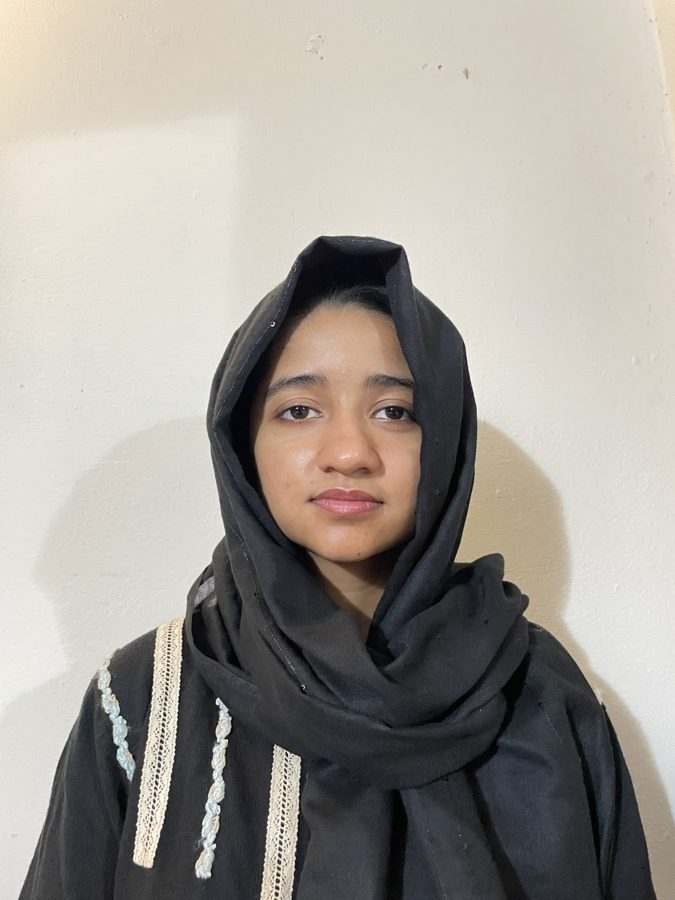
\includegraphics[width=\linewidth]{figures/sample_scarf.jpg}\caption*{Scarf}\end{minipage}\hfill
\begin{minipage}{0.24\textwidth}\centering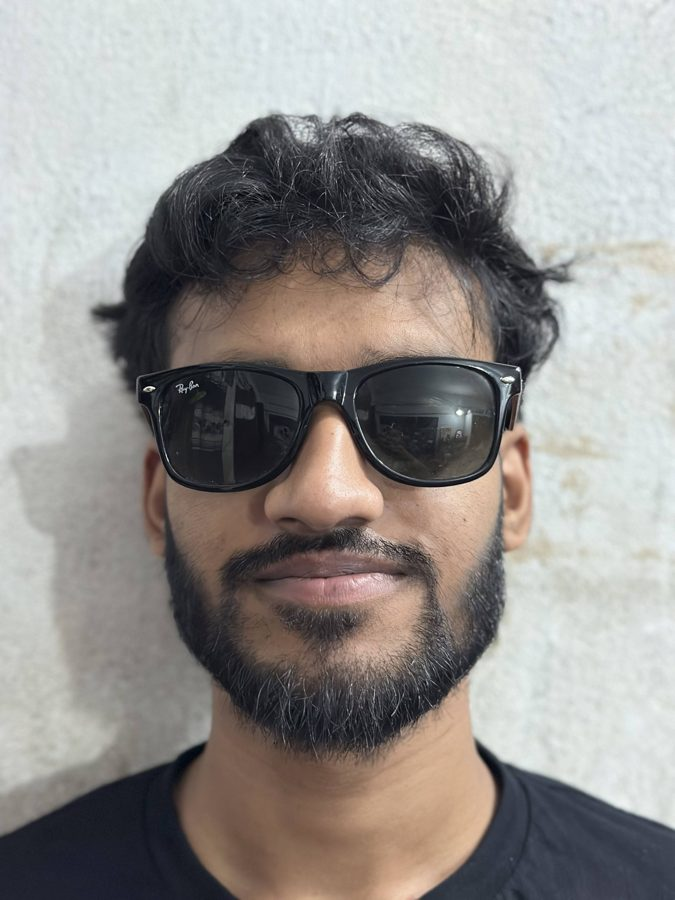
\includegraphics[width=\linewidth]{figures/sample_sunglass.jpg}\caption*{Sunglasses}\end{minipage}\hfill
\begin{minipage}{0.24\textwidth}\centering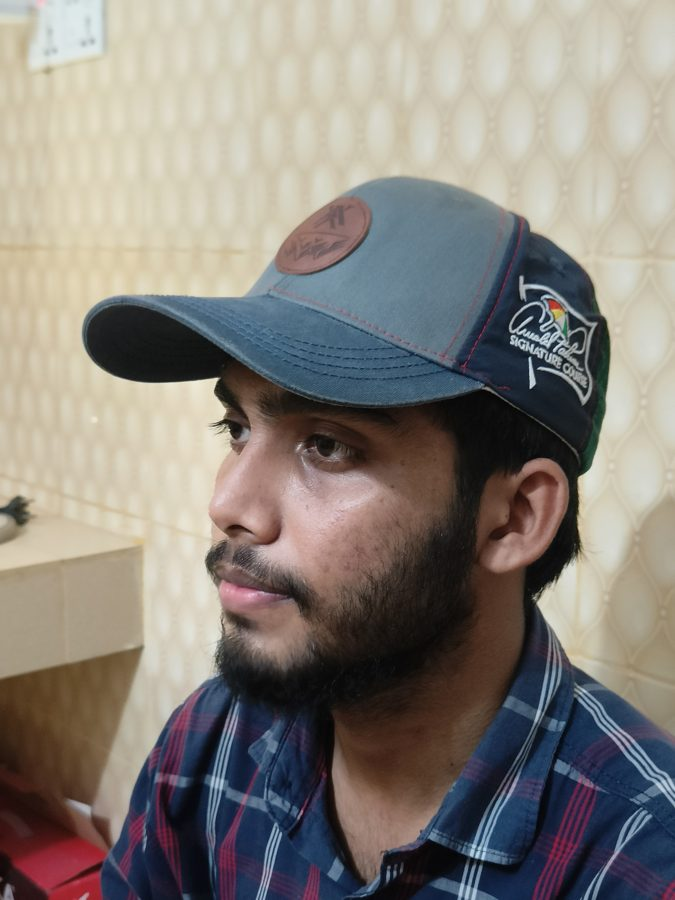
\includegraphics[width=\linewidth]{figures/sample_cap.jpg}\caption*{Cap}\end{minipage}\hfill
\begin{minipage}{0.24\textwidth}\centering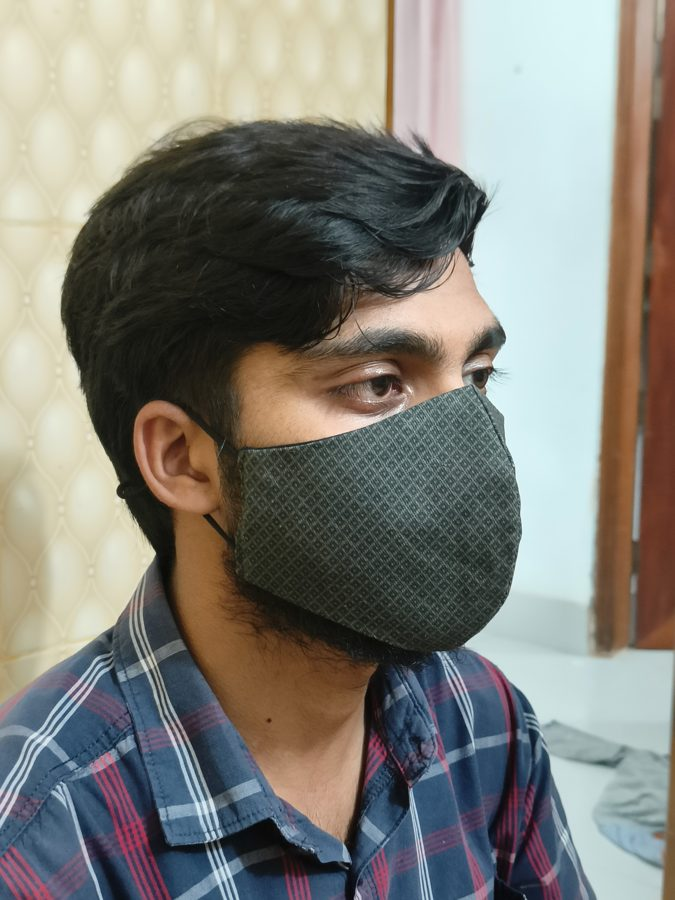
\includegraphics[width=\linewidth]{figures/sample_mask.jpg}\caption*{Mask}\end{minipage}
\caption{Real accepted samples, one per occlusion family (participants who ticked the optional photo-permission box).}
\label{fig:sample-accepted}
\end{figure}

\begin{figure}[htbp]
\centering
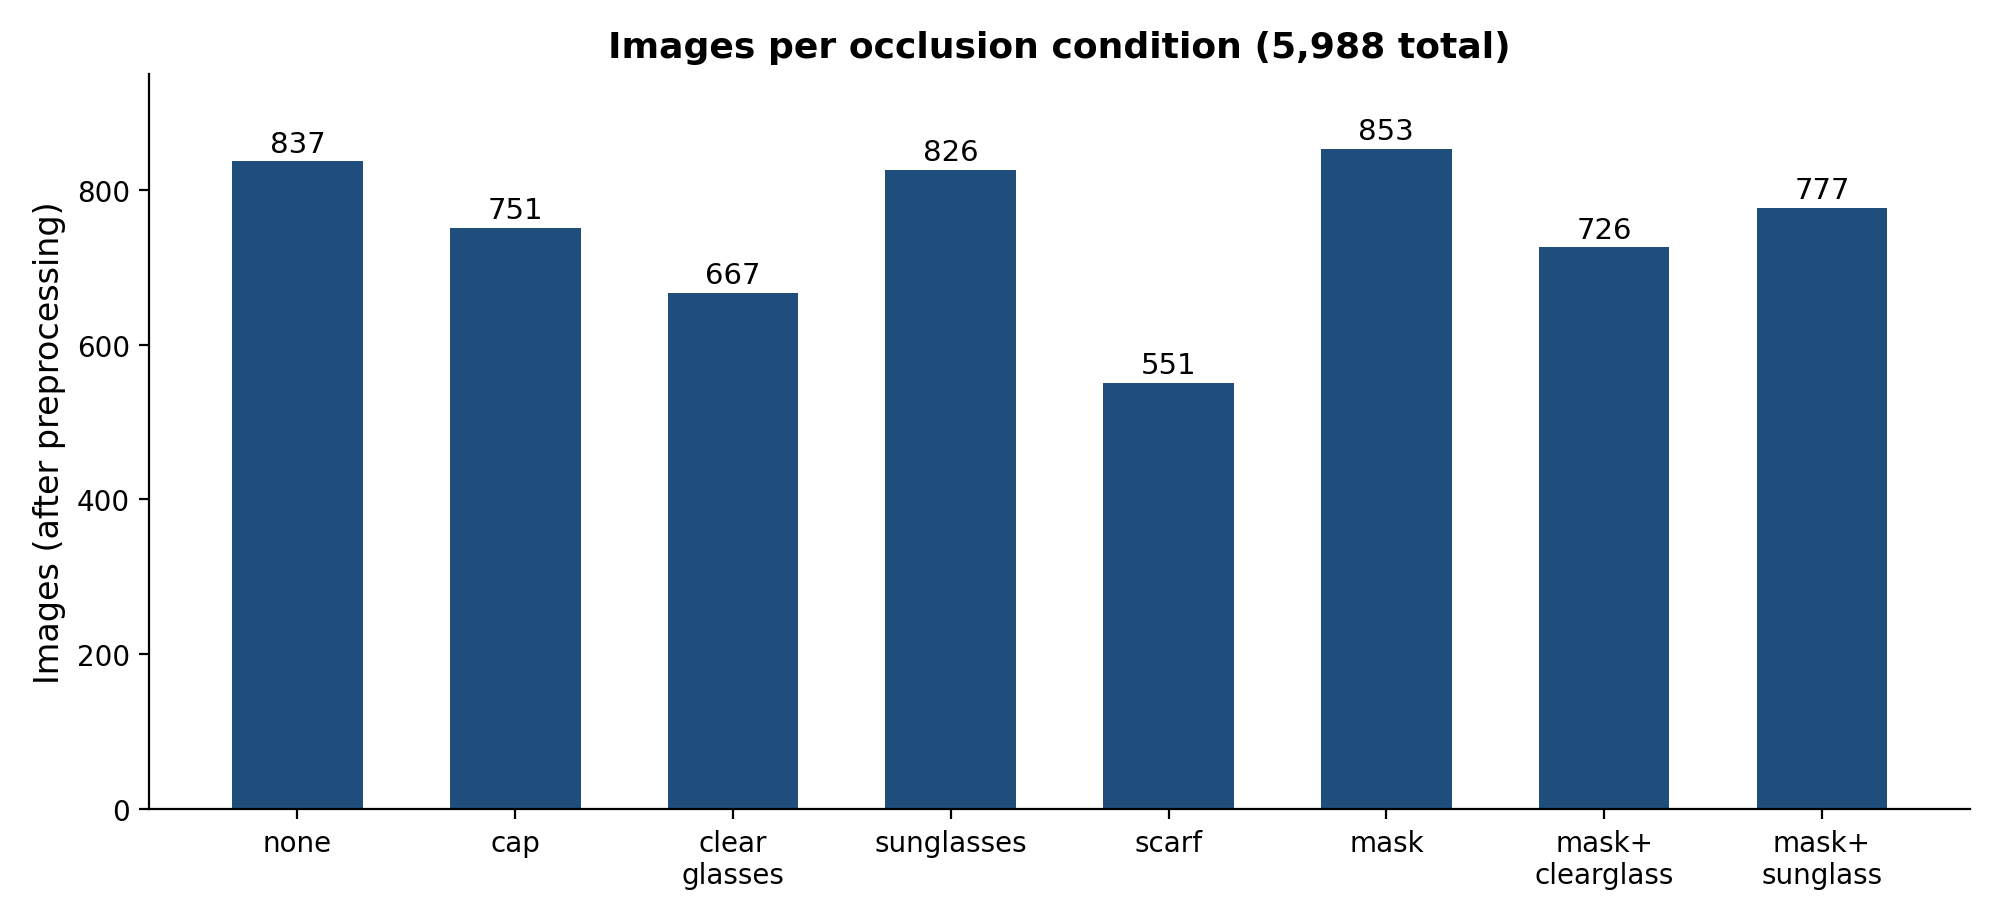
\includegraphics[width=0.85\linewidth]{figures/chart_per_occlusion_counts.png}
\caption{Number of images per occlusion condition after preprocessing (5{,}988 total).}
\label{fig:occ-counts}
\end{figure}

\subsection{A Note on Synthetic Images}
\label{sec:synthetic}

The large majority of the dataset is real captured photographs: every identity was photographed wearing every occlusion condition in person. A small minority of images are an exception: a handful of participants declined to physically wear a specific occlusion (most often sunglasses, for personal or religious reasons), so a synthetic version of that occlusion was digitally added to one of their clean photos instead, purely so that identity's coverage of that condition would not be entirely missing. These synthetic images are a small fraction of the dataset and are not separately flagged in the manifest, so their exact count is not reported here; the intent is full disclosure that they exist, not a claim that they are common.

Beyond this, the training-only augmentation pipeline (Section~\ref{sec:model}) applies mild synthetic transformations --- horizontal flips, small rotations, brightness/contrast jitter, resolution degradation, motion/Gaussian blur, sensor noise, JPEG re-compression, and random erasing --- to simulate the live phone-camera domain the deployed demo runs in. These are training-time-only variations of real photos, not new synthetic identities or occlusions.

\section{Data Cleaning and Quality Control}
\label{sec:cleaning}

Photos were rejected (and moved to a separate \texttt{put\_asides} folder with a recorded reason, never silently deleted) for: excessive blur, unusable low light, a face fully covered with no identity-bearing region left visible, or bad framing/cropping. Figure~\ref{fig:sample-rejected} shows one real rejected example for each reason. This project's dataset is treated as \textbf{fixed} as of the start of the training phase --- no further deletions, restorations, or relabelling were performed once preprocessing began, so every number in this report is computed on the same frozen 6{,}000-image set.

\begin{figure}[htbp]
\centering
\begin{minipage}{0.24\textwidth}\centering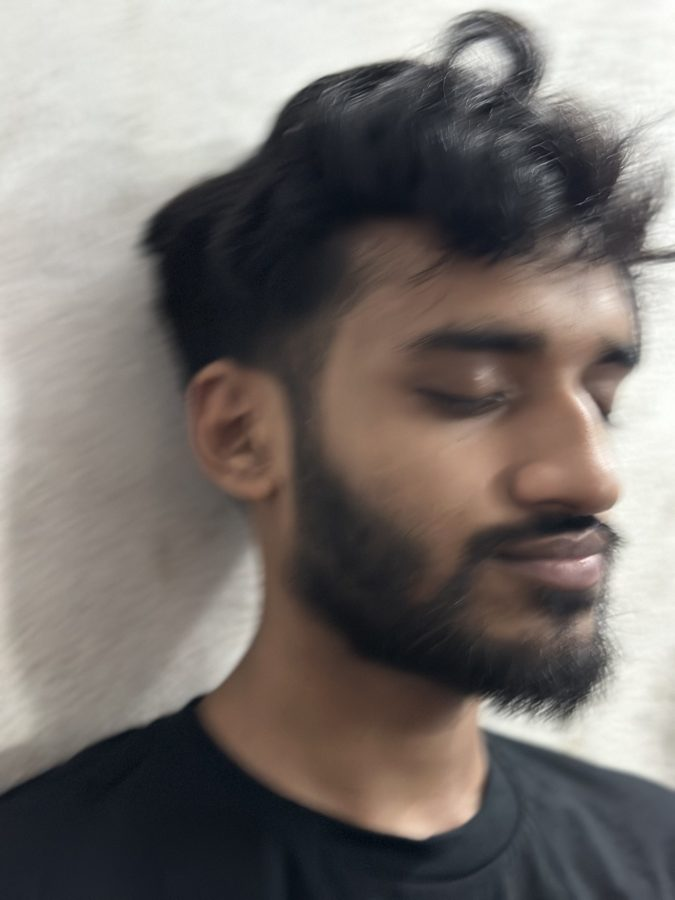
\includegraphics[width=\linewidth]{figures/reject_blurred.jpg}\caption*{Too blurry}\end{minipage}\hfill
\begin{minipage}{0.24\textwidth}\centering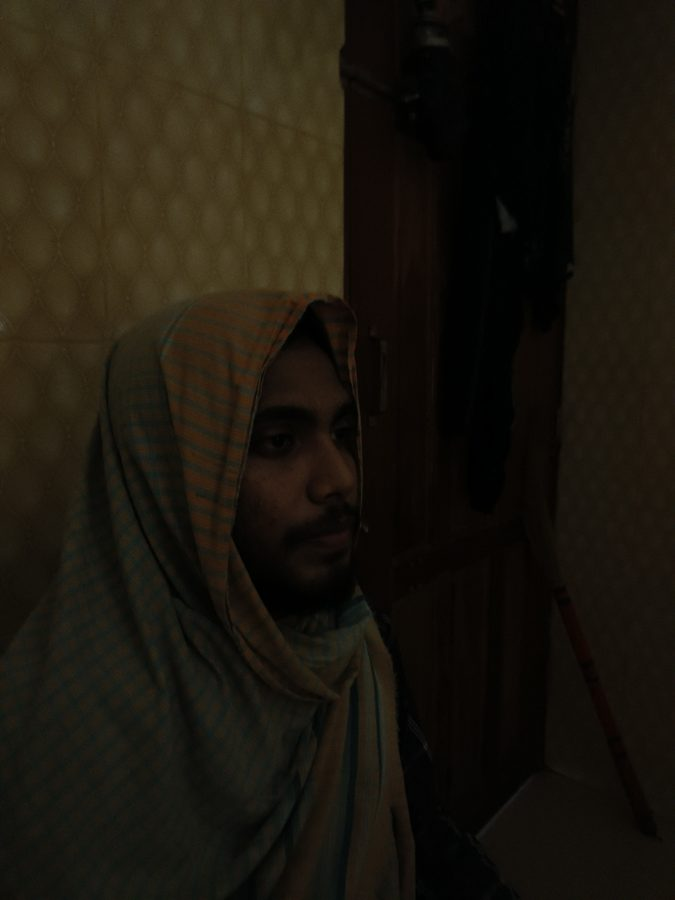
\includegraphics[width=\linewidth]{figures/reject_lowlight.jpg}\caption*{Too dark}\end{minipage}\hfill
\begin{minipage}{0.24\textwidth}\centering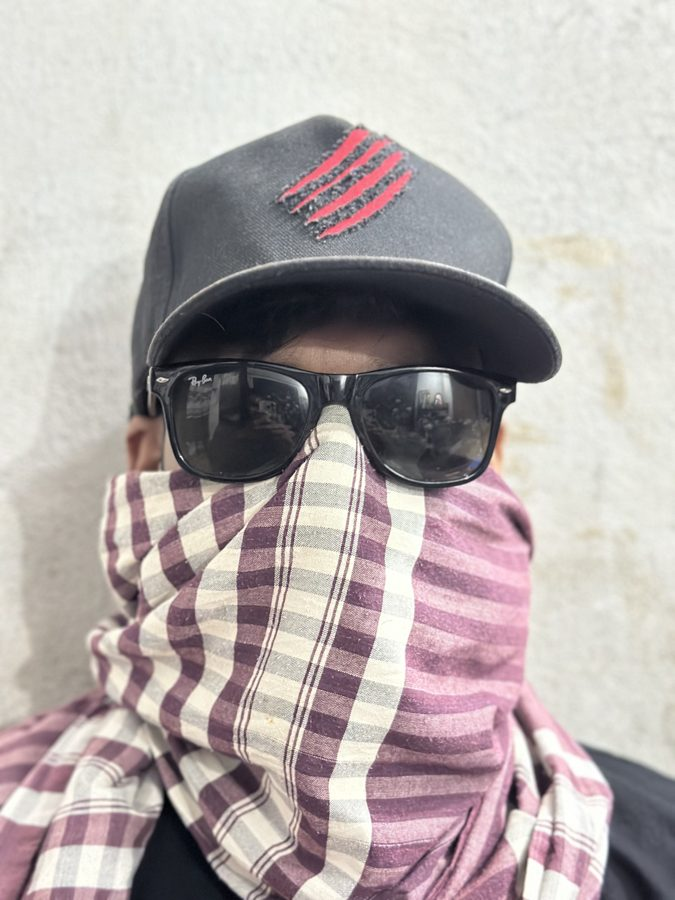
\includegraphics[width=\linewidth]{figures/reject_covered.jpg}\caption*{Fully covered}\end{minipage}\hfill
\begin{minipage}{0.24\textwidth}\centering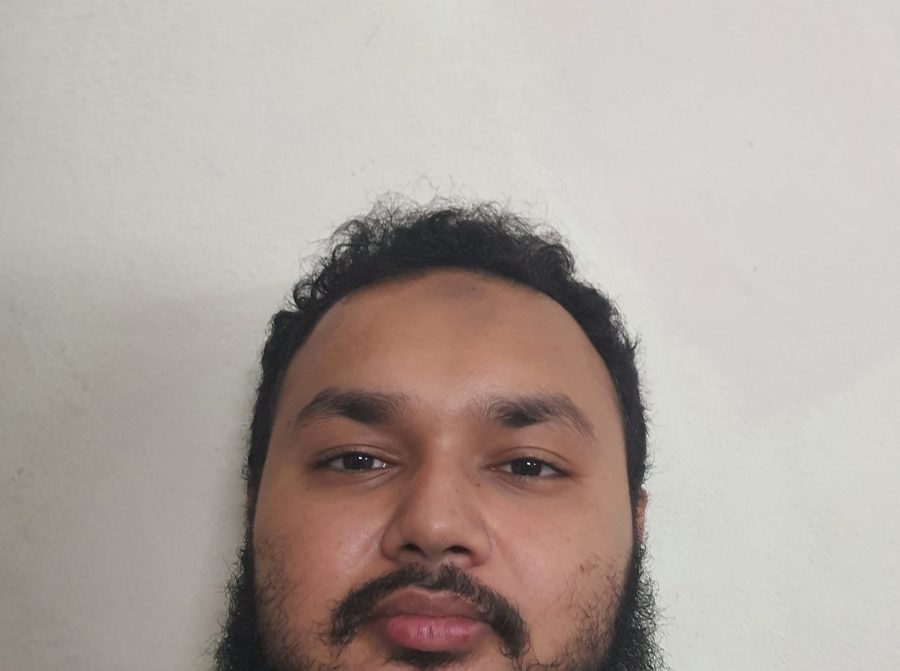
\includegraphics[width=\linewidth]{figures/reject_miscropped.jpg}\caption*{Mis-cropped}\end{minipage}
\caption{Real rejected samples, one per quality-control reason.}
\label{fig:sample-rejected}
\end{figure}

\section{Data Preprocessing}
\label{sec:preprocessing}

Every accepted photo passes through one fixed pipeline (\texttt{scripts/01\_preprocess.py}), identical for training, validation, test, and later, the live demo. Figure~\ref{fig:preprocess-pipeline} shows the flow.

\begin{figure}[htbp]
\centering
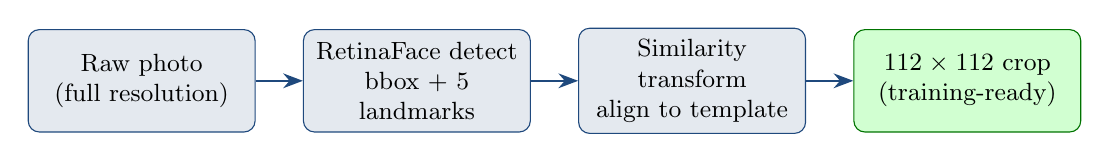
\begin{tikzpicture}[node distance=0.6cm]
\node[pbox] (raw) {Raw photo\\(full resolution)};
\node[pbox, right=of raw] (det) {RetinaFace detect\\bbox + 5 landmarks};
\node[pbox, right=of det] (align) {Similarity transform\\align to template};
\node[pboxend, right=of align] (crop) {$112\times112$ crop\\(training-ready)};
\draw[parrow] (raw) -- (det);
\draw[parrow] (det) -- (align);
\draw[parrow] (align) -- (crop);
\end{tikzpicture}
\caption{Preprocessing pipeline: every accepted photo, before it can be used for training, evaluation, or live inference.}
\label{fig:preprocess-pipeline}
\end{figure}

\begin{enumerate}[label=\arabic*.]
\item \textbf{Detect.} RetinaFace (\texttt{insightface}'s \texttt{buffalo\_l} detector, \texttt{det\_10g.onnx}) locates the face and its five landmarks (both eyes, nose, both mouth corners) at \texttt{det\_size=(640,640)}, \texttt{det\_thresh=0.5}. The largest detected face is kept.
\item \textbf{Fallback on failure.} If nothing is detected, the image is retried at a looser \texttt{det\_thresh=0.3}, and if that still fails, at 2$\times$ upscale with the loose threshold. Every failure is logged, never dropped silently.
\item \textbf{Align and crop.} A similarity transform (\texttt{insightface.utils.face\_align.norm\_crop}) maps the five landmarks onto ArcFace's standard reference template, producing a $112\times112$ aligned crop. This step is what prevents the classifier from keying on background or camera artifacts rather than the face.
\item \textbf{Log.} Each image's path, identity, occlusion, lighting, source filename, MD5 hash, detection outcome/score/stage, and crop path are appended to \texttt{metadata/preprocess\_log.csv}.
\end{enumerate}

\textbf{Result:} 5{,}988 of 6{,}000 images (99.8\%) were successfully detected and aligned, comfortably above the 97\% acceptance gate set in the training plan. The 12 failures were concentrated in the hardest occlusion conditions --- 10 in \texttt{mask\_sunglass} and 2 in \texttt{mask} --- where the combination of a covered lower face and (for 10 of them) a covered eye region left too little visible structure for landmark detection even at the loosened threshold.

\section{Data Organisation and Split}
\label{sec:split}

\subsection{Group-Aware Splitting}

Splitting is not simple random assignment, because near-duplicate images are a real risk: a burst of photos taken a few seconds apart, or a low-light image derived by darkening a regular-light one, could otherwise land on opposite sides of the split and make test accuracy look better than genuine generalisation. (A small number of exact, byte-identical duplicate photos also exist in the raw capture, from repeat shutter presses; these are treated as independent images like any other, and every MD5 hash is logged during preprocessing so this stays auditable.) Two images are grouped together (and therefore forced into the same split) if:
\begin{itemize}
\item they are derived from the same source image (e.g.\ a brightness-adjusted low-light pair), or
\item they belong to the same person \emph{and} the same occlusion, and were captured within a 10-second window of each other, with burst-chains capped at an 8-second total span to prevent one long shooting burst from silently swallowing an entire occlusion condition for a participant.
\end{itemize}
Groups are then assigned, as whole units, to train/validation/test using a deficit-based greedy allocator: the largest groups are placed first, each into whichever split currently has the largest shortfall relative to its 60/20/20 target share, computed independently per (person, occlusion) cell. This avoids the naive failure mode of a simple sequential fill, which was observed during development to produce a wildly unbalanced split (train 24\%, val 58\%, test 18\%) when a single 49-image group was assigned in one step.

\subsection{Coverage Guarantee}

A hard requirement was enforced: \textbf{every one of the 30 participants must appear in all three splits.} A repair pass exists to forcibly move whole groups from train into an under-represented split if the natural allocation leaves any participant below a floor of 2 images per split; in the final run this repair pass was not needed. Per-occlusion coverage within each split was treated as best-effort rather than a hard requirement: 36 of 240 (person $\times$ occlusion) cells are absent from the test split specifically (informational only, not a failure condition).

\subsection{Final Split}

\begin{table}[h]
\centering
\caption{Final train/validation/test split (5{,}988 successfully preprocessed images).}
\begin{tabular}{lrr}
\toprule
\textbf{Split} & \textbf{Images} & \textbf{Share} \\
\midrule
Train & 3{,}546 & 59\% \\
Validation & 1{,}444 & 24\% \\
Test & 998 & 17\% \\
\midrule
\textbf{Total} & \textbf{5{,}988} & 100\% \\
\bottomrule
\end{tabular}
\end{table}

All hard assertions (no group spans two splits; every participant in all three splits) passed on this final assignment.

\section{Model and Training Approach}
\label{sec:model}

\subsection{Selected Models}

\begin{itemize}
\item \textbf{RetinaFace} \cite{deng2020retinaface} (\texttt{det\_10g.onnx}) — detection and five-point landmark alignment (Section~\ref{sec:preprocessing}).
\item \textbf{Pretrained ArcFace} \cite{deng2019arcface}, iResNet50 backbone (\texttt{w600k\_r50.onnx}, \texttt{insightface} \texttt{buffalo\_l}) — turns each aligned $112\times112$ crop into a 512-dimensional embedding. This is the primary identification model in every experiment below.
\end{itemize}

RetinaFace and ArcFace were selected, as in the proposal, because they are purpose-built for faces, need far less local data than training from scratch, are light enough to run on both a 2$\times$RTX~3090 remote box and later a modest laptop CPU, and have precedent in prior published work adapting the same family to occluded/masked faces (Section~\ref{sec:related}). Unlike the proposal, no separate from-scratch CNN baseline was trained: with only 30 classes and a few hundred images per identity, a from-scratch CNN was judged inherently weaker than adapting a large-scale pretrained backbone, and unlikely to add an informative data point — effort was redirected to a more informative fine-tuning ladder (E1--E3 below).

\subsection{Experiments}

Three experiments were run, each answering a specific question about how much task-specific training the pretrained embedding actually needs:

\begin{table}[h]
\centering
\caption{Experiment design.}
\begin{tabular}{L{1cm}L{3cm}L{3.6cm}L{6cm}}
\toprule
\textbf{ID} & \textbf{Name} & \textbf{Backbone} & \textbf{Question} \\
\midrule
E1 & Trained head, clean-only & Frozen + new identity head & The proposal's original baseline: train only on the \texttt{none} condition. \\
E2 & Trained head, mixed-condition & Frozen + new identity head & Does training on all eight occlusion conditions help over E1? \\
E3 & Partial backbone fine-tune & Last 15\% of backbone unfrozen + head & Does adapting backbone weights (not just the head) help further? \\
\bottomrule
\end{tabular}
\end{table}

\textbf{E1 and E2} keep the entire pretrained ArcFace backbone frozen and train only a new, small classification layer on top of it that learns to tell the 30 enrolled identities apart. The two experiments are identical in every setting except their training data: E1 only ever sees clean, unoccluded faces during training, while E2 sees all eight occlusion conditions. Both use a standard identity-margin training objective (the same family of loss ArcFace itself was trained with) and are trained with the AdamW optimiser. Figure~\ref{fig:pipeline-e1e2} shows the pipeline.

\begin{figure}[htbp]
\centering
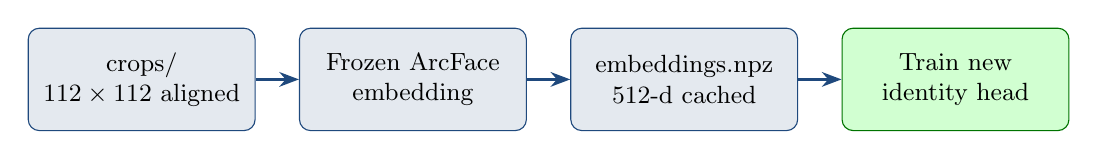
\begin{tikzpicture}[node distance=0.55cm]
\node[pbox] (crop) {crops/\\$112\times112$ aligned};
\node[pbox, right=of crop] (embed) {Frozen ArcFace\\embedding};
\node[pbox, right=of embed] (cache) {embeddings.npz\\512-d cached};
\node[pboxend, right=of cache] (head) {Train new\\identity head};
\draw[parrow] (crop) -- (embed);
\draw[parrow] (embed) -- (cache);
\draw[parrow] (cache) -- (head);
\end{tikzpicture}
\caption{E1/E2 training pipeline. The only difference between the two runs is which images are shown to the ``train new identity head'' step.}
\label{fig:pipeline-e1e2}
\end{figure}

\textbf{E3} goes a step further and allows the last 15\% of the backbone's own parameters to be updated as well, in addition to training a new identity head, so the network can slightly adjust its own face representation rather than only fitting a decision boundary on top of a fixed one. Only the last layers are unfrozen (not the whole network) because with only a few thousand training images, adjusting the entire backbone risks overwriting the general face knowledge it already has; the layers closest to the output are also the ones that encode the most identity-specific detail, making them the most useful ones to adapt. The internal statistics that batch-normalisation layers rely on are kept frozen throughout training as well, since updating them on so few images was found to quietly degrade the pretrained features. Because \texttt{insightface} ships ArcFace only as a ready-to-run inference package with no trainable copy available, the backbone was converted into a trainable form and checked against the original to confirm it behaves identically (outputs matched to better than four decimal places) before any training took place, so E3 is a genuine adjustment of the original pretrained weights rather than a stand-in model. Figure~\ref{fig:pipeline-e3} shows the pipeline.

\begin{figure}[htbp]
\centering
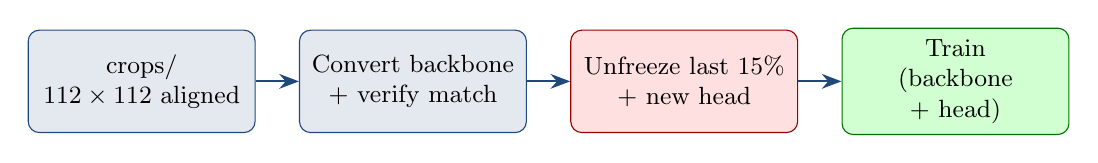
\begin{tikzpicture}[node distance=0.55cm]
\node[pbox] (crop) {crops/\\$112\times112$ aligned};
\node[pbox, right=of crop] (conv) {Convert backbone\\+ verify match};
\node[pboxwarn, right=of conv] (unfreeze) {Unfreeze last 15\%\\+ new head};
\node[pboxend, right=of unfreeze] (train) {Train\\(backbone + head)};
\draw[parrow] (crop) -- (conv);
\draw[parrow] (conv) -- (unfreeze);
\draw[parrow] (unfreeze) -- (train);
\end{tikzpicture}
\caption{E3 training pipeline. Unlike E1/E2, raw crops are needed again here (not just cached embeddings), since gradients must flow back through the backbone itself.}
\label{fig:pipeline-e3}
\end{figure}

\textbf{How the validation split was actually used.} The validation set never contributes to any reported accuracy number, but it does two jobs during training. First, it decides when to stop: after every training pass, each model's performance is checked on validation data, and training stops once that stops improving, so the model is not simply memorising the training images for longer than necessary. Second, it was the basis for choosing settings while building the pipeline -- for example, how strongly to weight the identity margin, what learning rate the head versus the backbone should use in E3, and how large a slice of the backbone to unfreeze -- by comparing validation performance across a few candidate settings before committing to one and only then measuring test accuracy. Test data was never looked at during any of this.

No augmentation was applied to validation or test data at any stage; the live-capture-style augmentations described in Section~\ref{sec:synthetic} were applied only to E1/E2/E3 training images.

\section{Results}
\label{sec:results}

Because every identity contributes an equal, fixed share of the dataset (Section~\ref{sec:dataset}), plain top-1 accuracy is already a fair, sufficient headline number overall. Within a single occlusion condition, though, one accuracy number can hide \emph{which} identities are driving the errors, so the per-occlusion breakdown below reports precision, recall, and F1 per condition instead: for each occlusion, the test images restricted to that condition are used to compute standard multi-class precision/recall/F1 across the 30 identities, so a condition's precision specifically penalises identities being over-predicted within that occlusion, not merely misclassified. Each experiment was evaluated with a dedicated script (\texttt{scripts/10\_full\_eval.py}) that also computes a full $30\times30$ confusion matrix, kept as a reusable CSV/PNG artifact under \texttt{runs/eval/<experiment>/}.

\begin{table}[h]
\centering
\caption{Test-set top-1 accuracy across all three experiments (998 test images, 30 balanced classes).}
\begin{tabular}{lr}
\toprule
\textbf{Experiment} & \textbf{Top-1 accuracy} \\
\midrule
E1 — Head, clean-only & 94.29\% \\
E2 — Head, mixed-condition & 99.90\% \\
E3 — Partial backbone fine-tune & \textbf{100.00\%} \\
\bottomrule
\end{tabular}
\end{table}

\begin{table}[h]
\centering
\footnotesize
\caption{Per-occlusion precision (P), recall (R), and F1, across all three experiments, showing exactly where each approach's remaining errors are concentrated. Each triple is computed only from that occlusion's test images.}
\begin{tabular}{lr ccc ccc ccc}
\toprule
& & \multicolumn{3}{c}{\textbf{E1}} & \multicolumn{3}{c}{\textbf{E2}} & \multicolumn{3}{c}{\textbf{E3}} \\
\cmidrule(lr){3-5}\cmidrule(lr){6-8}\cmidrule(lr){9-11}
\textbf{Occlusion} & \textbf{n} & P & R & F1 & P & R & F1 & P & R & F1 \\
\midrule
none               & 138 & 100.0 & 100.0 & 100.0 & 100.0 & 100.0 & 100.0 & 100.0 & 100.0 & 100.0 \\
cap                & 129 & 100.0 & 100.0 & 100.0 & 100.0 & 100.0 & 100.0 & 100.0 & 100.0 & 100.0 \\
clear glasses      & 108 & 100.0 & 100.0 & 100.0 & 100.0 & 100.0 & 100.0 & 100.0 & 100.0 & 100.0 \\
sunglasses         & 125 & 100.0 & 100.0 & 100.0 & 100.0 & 100.0 & 100.0 & 100.0 & 100.0 & 100.0 \\
scarf              &  84 &  97.4 &  96.3 &  96.8 & 100.0 & 100.0 & 100.0 & 100.0 & 100.0 & 100.0 \\
mask               & 161 &  97.3 &  96.0 &  95.8 &  99.5 &  99.4 &  99.4 & 100.0 & 100.0 & 100.0 \\
mask+clear glasses & 120 &  87.6 &  86.4 &  85.8 & 100.0 & 100.0 & 100.0 & 100.0 & 100.0 & 100.0 \\
mask+sunglasses    & 133 &  \textbf{75.5} &  \textbf{71.4} &  \textbf{68.9} & 100.0 & 100.0 & 100.0 & 100.0 & 100.0 & 100.0 \\
\bottomrule
\end{tabular}
\end{table}

\textbf{E1 vs.\ E2 is the clearest and most informative comparison in this report.} A head trained only on clean, unoccluded faces (E1) drops to 75.5\% precision / 71.4\% recall / 68.9\% F1 specifically on the hardest combined condition, \texttt{mask+sunglasses} — the one occlusion pair that removes both the eye region and the lower face simultaneously — while still scoring a perfect 100.0\% across the board on every single-occlusion condition. The identical head trained on all eight conditions (E2) recovers to a perfect 100.0\% on that same condition (and 99.90\% top-1 overall). This is direct, quantitative evidence that occlusion-diverse training data specifically matters for compound occlusions, not for single occlusions, which a pretrained face embedding already handles reasonably well without any task-specific training at all.

\textbf{E3, partial backbone fine-tuning, reached 100.00\% top-1}, correctly classifying every one of the 998 test images across all 30 identities and all eight occlusion conditions. Since E2 was already at 99.90\%, E3's gain is small in absolute terms — the honest reading is that E3 closes the last remaining gap rather than solving a problem E2 left substantially open. With E2 and E3 both at or above 99.9\%, this dataset and task, as collected, does not have enough headroom left to strongly differentiate them from each other; the more informative scientific result in this report is the E1-vs-E2 occlusion-diversity comparison on \texttt{mask+sunglasses} above, not the marginal gap between E2 and E3.

\subsection{Confusion Matrices}

Figures~\ref{fig:confusion-e1} and~\ref{fig:confusion-e2} show the row-normalised $30\times30$ test confusion matrix for E1 and E2 (E3's is a perfect diagonal with zero off-diagonal cells, since it classified every test image correctly, and is omitted here as uninformative). E2 is visually a clean diagonal with only one isolated off-diagonal cell; E1's matrix is the only one with a visible, systematic error pattern, concentrated in a handful of identities under \texttt{mask+sunglasses}. The single most common confusion in E1 is participant \texttt{p06} misclassified as \texttt{p16} (6 of 998 test images), followed by \texttt{p16}$\to$\texttt{p11} (5 images) and \texttt{p27}$\to$\texttt{p11} (4 images) — a small number of identities whose combined-occlusion appearance the clean-only head could not separate, resolved entirely once occlusion-diverse training data was used (E2). Full $30\times30$ counts for every experiment (E1, E2, and E3) are kept in \texttt{runs/eval/<experiment>/confusion\_matrix.csv} for reference.

\begin{figure}[htbp]
\centering
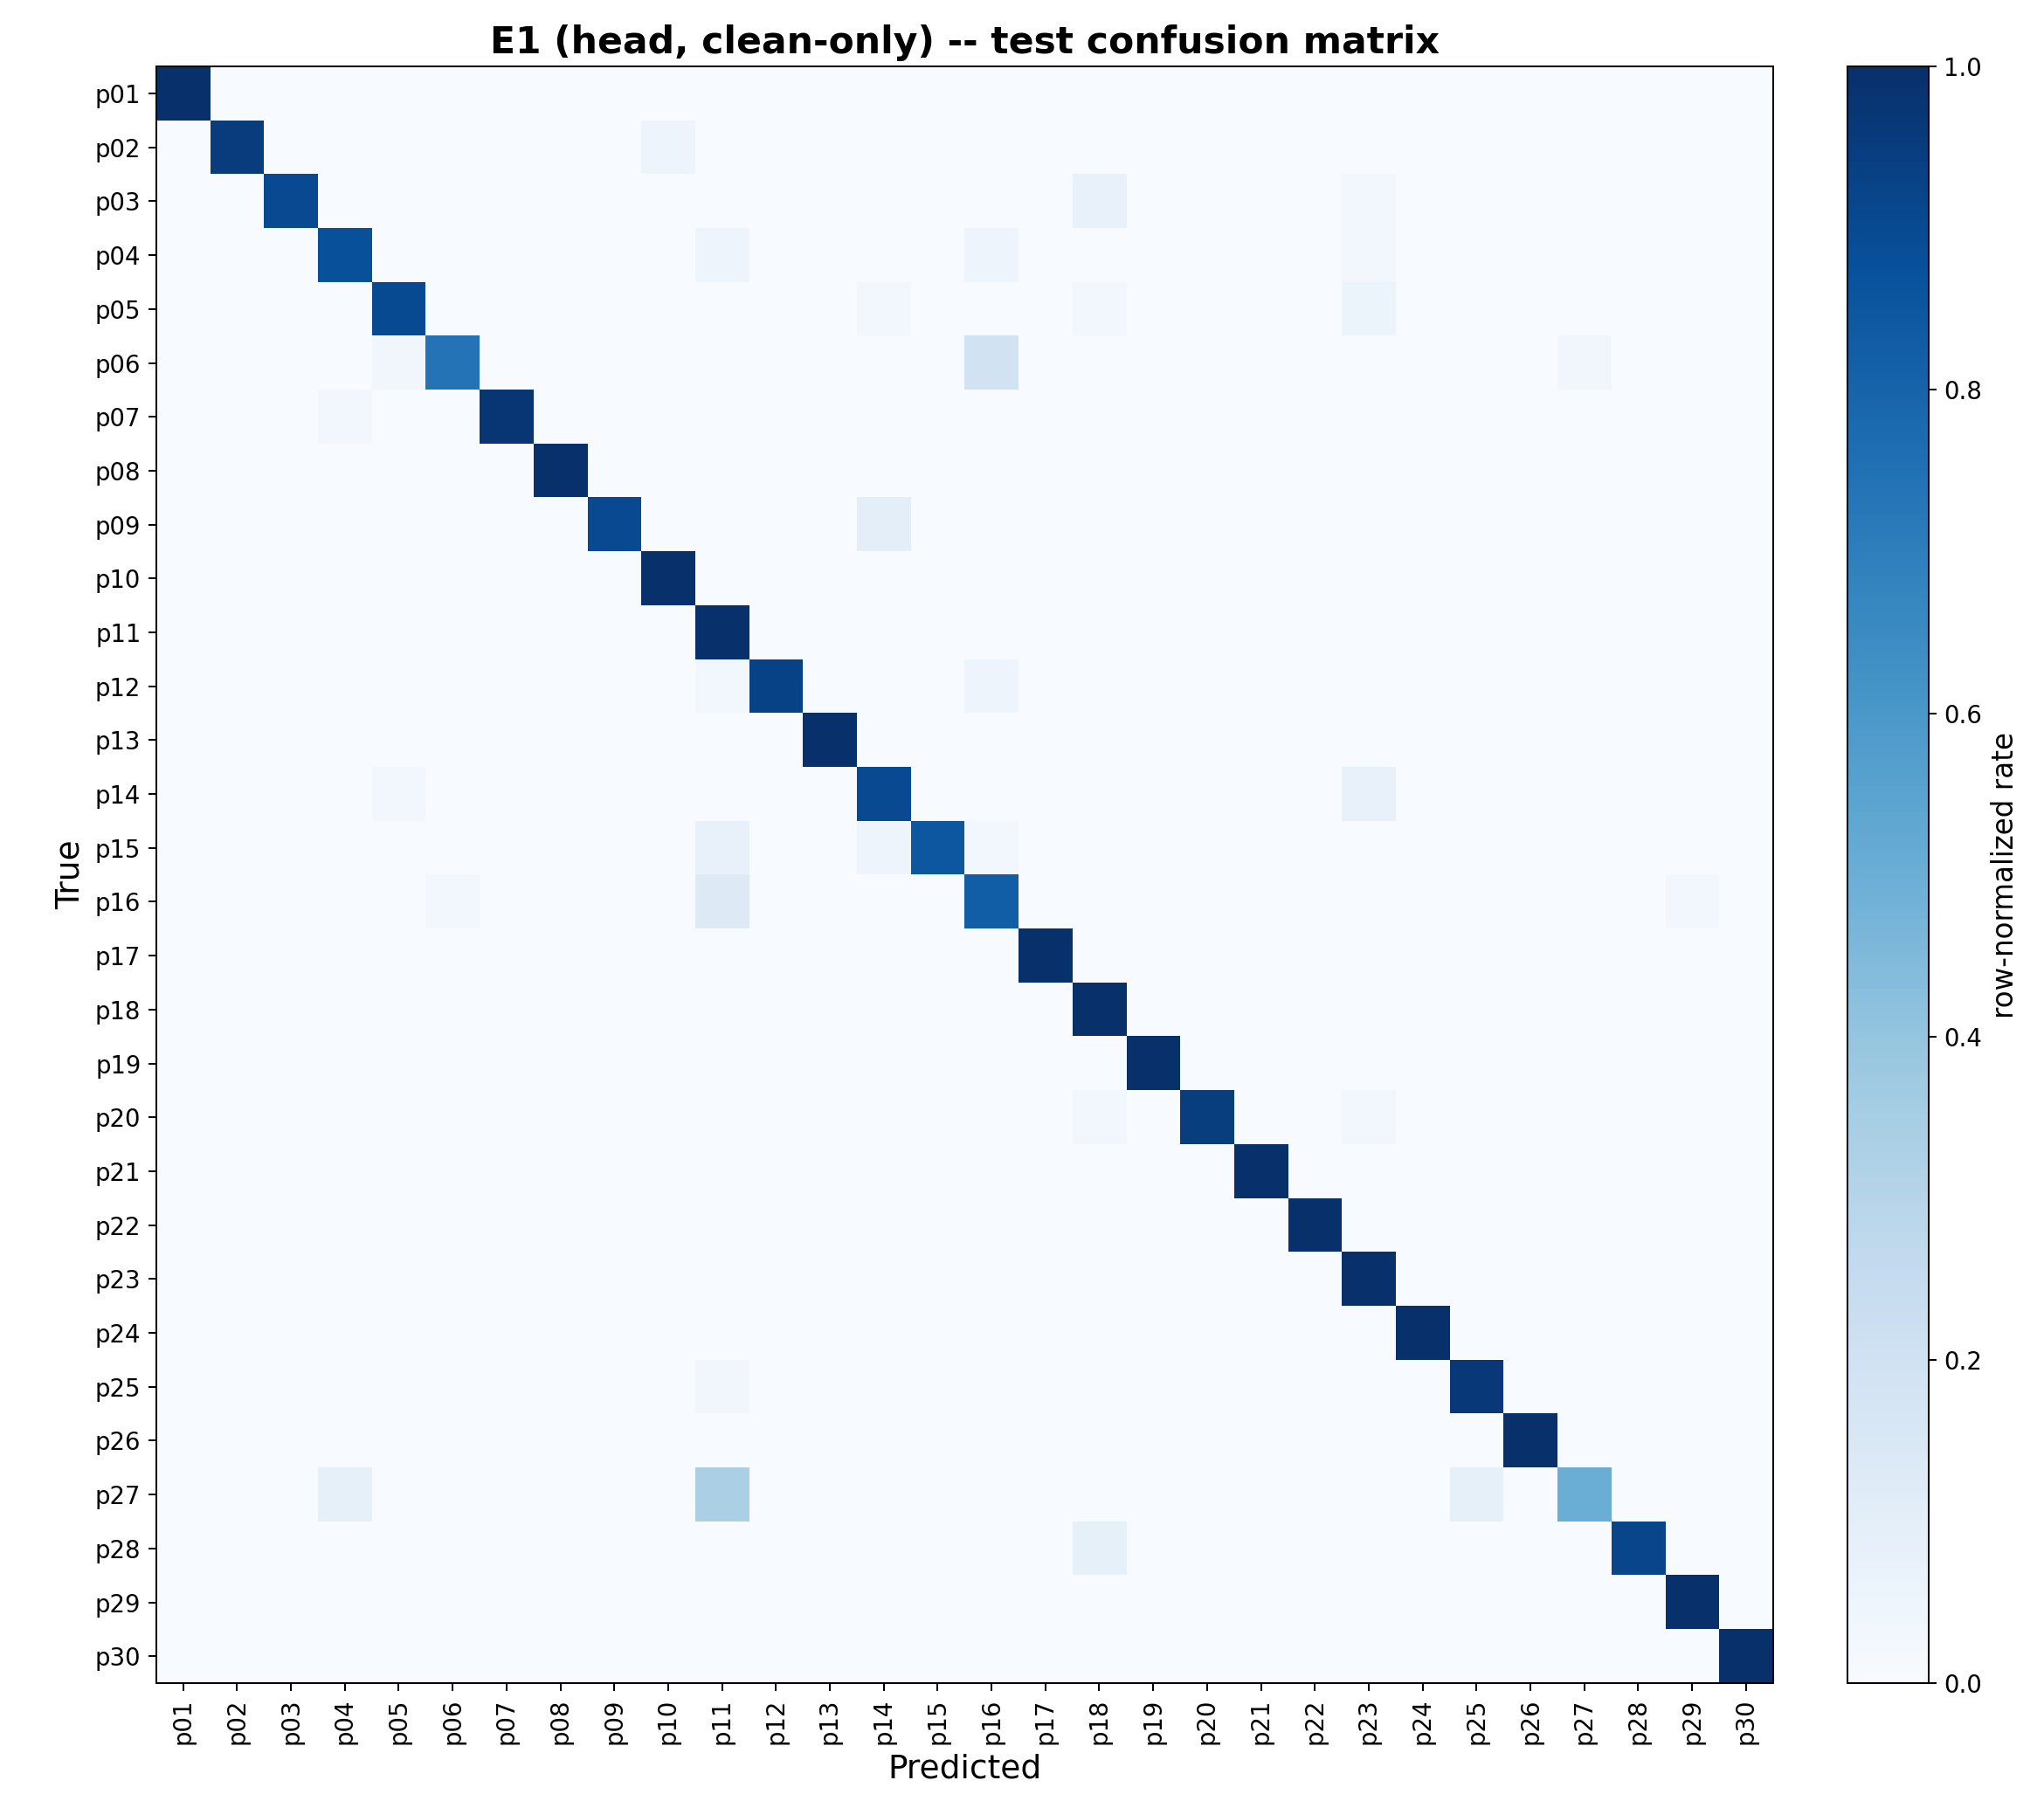
\includegraphics[width=0.92\linewidth]{figures/cm_large_e1.png}
\caption{Row-normalised $30\times30$ test confusion matrix, E1 (head, clean-only). Darker cells indicate a higher share of that identity's test images landing in that predicted column; a perfect classifier is a solid diagonal.}
\label{fig:confusion-e1}
\end{figure}

\begin{figure}[htbp]
\centering
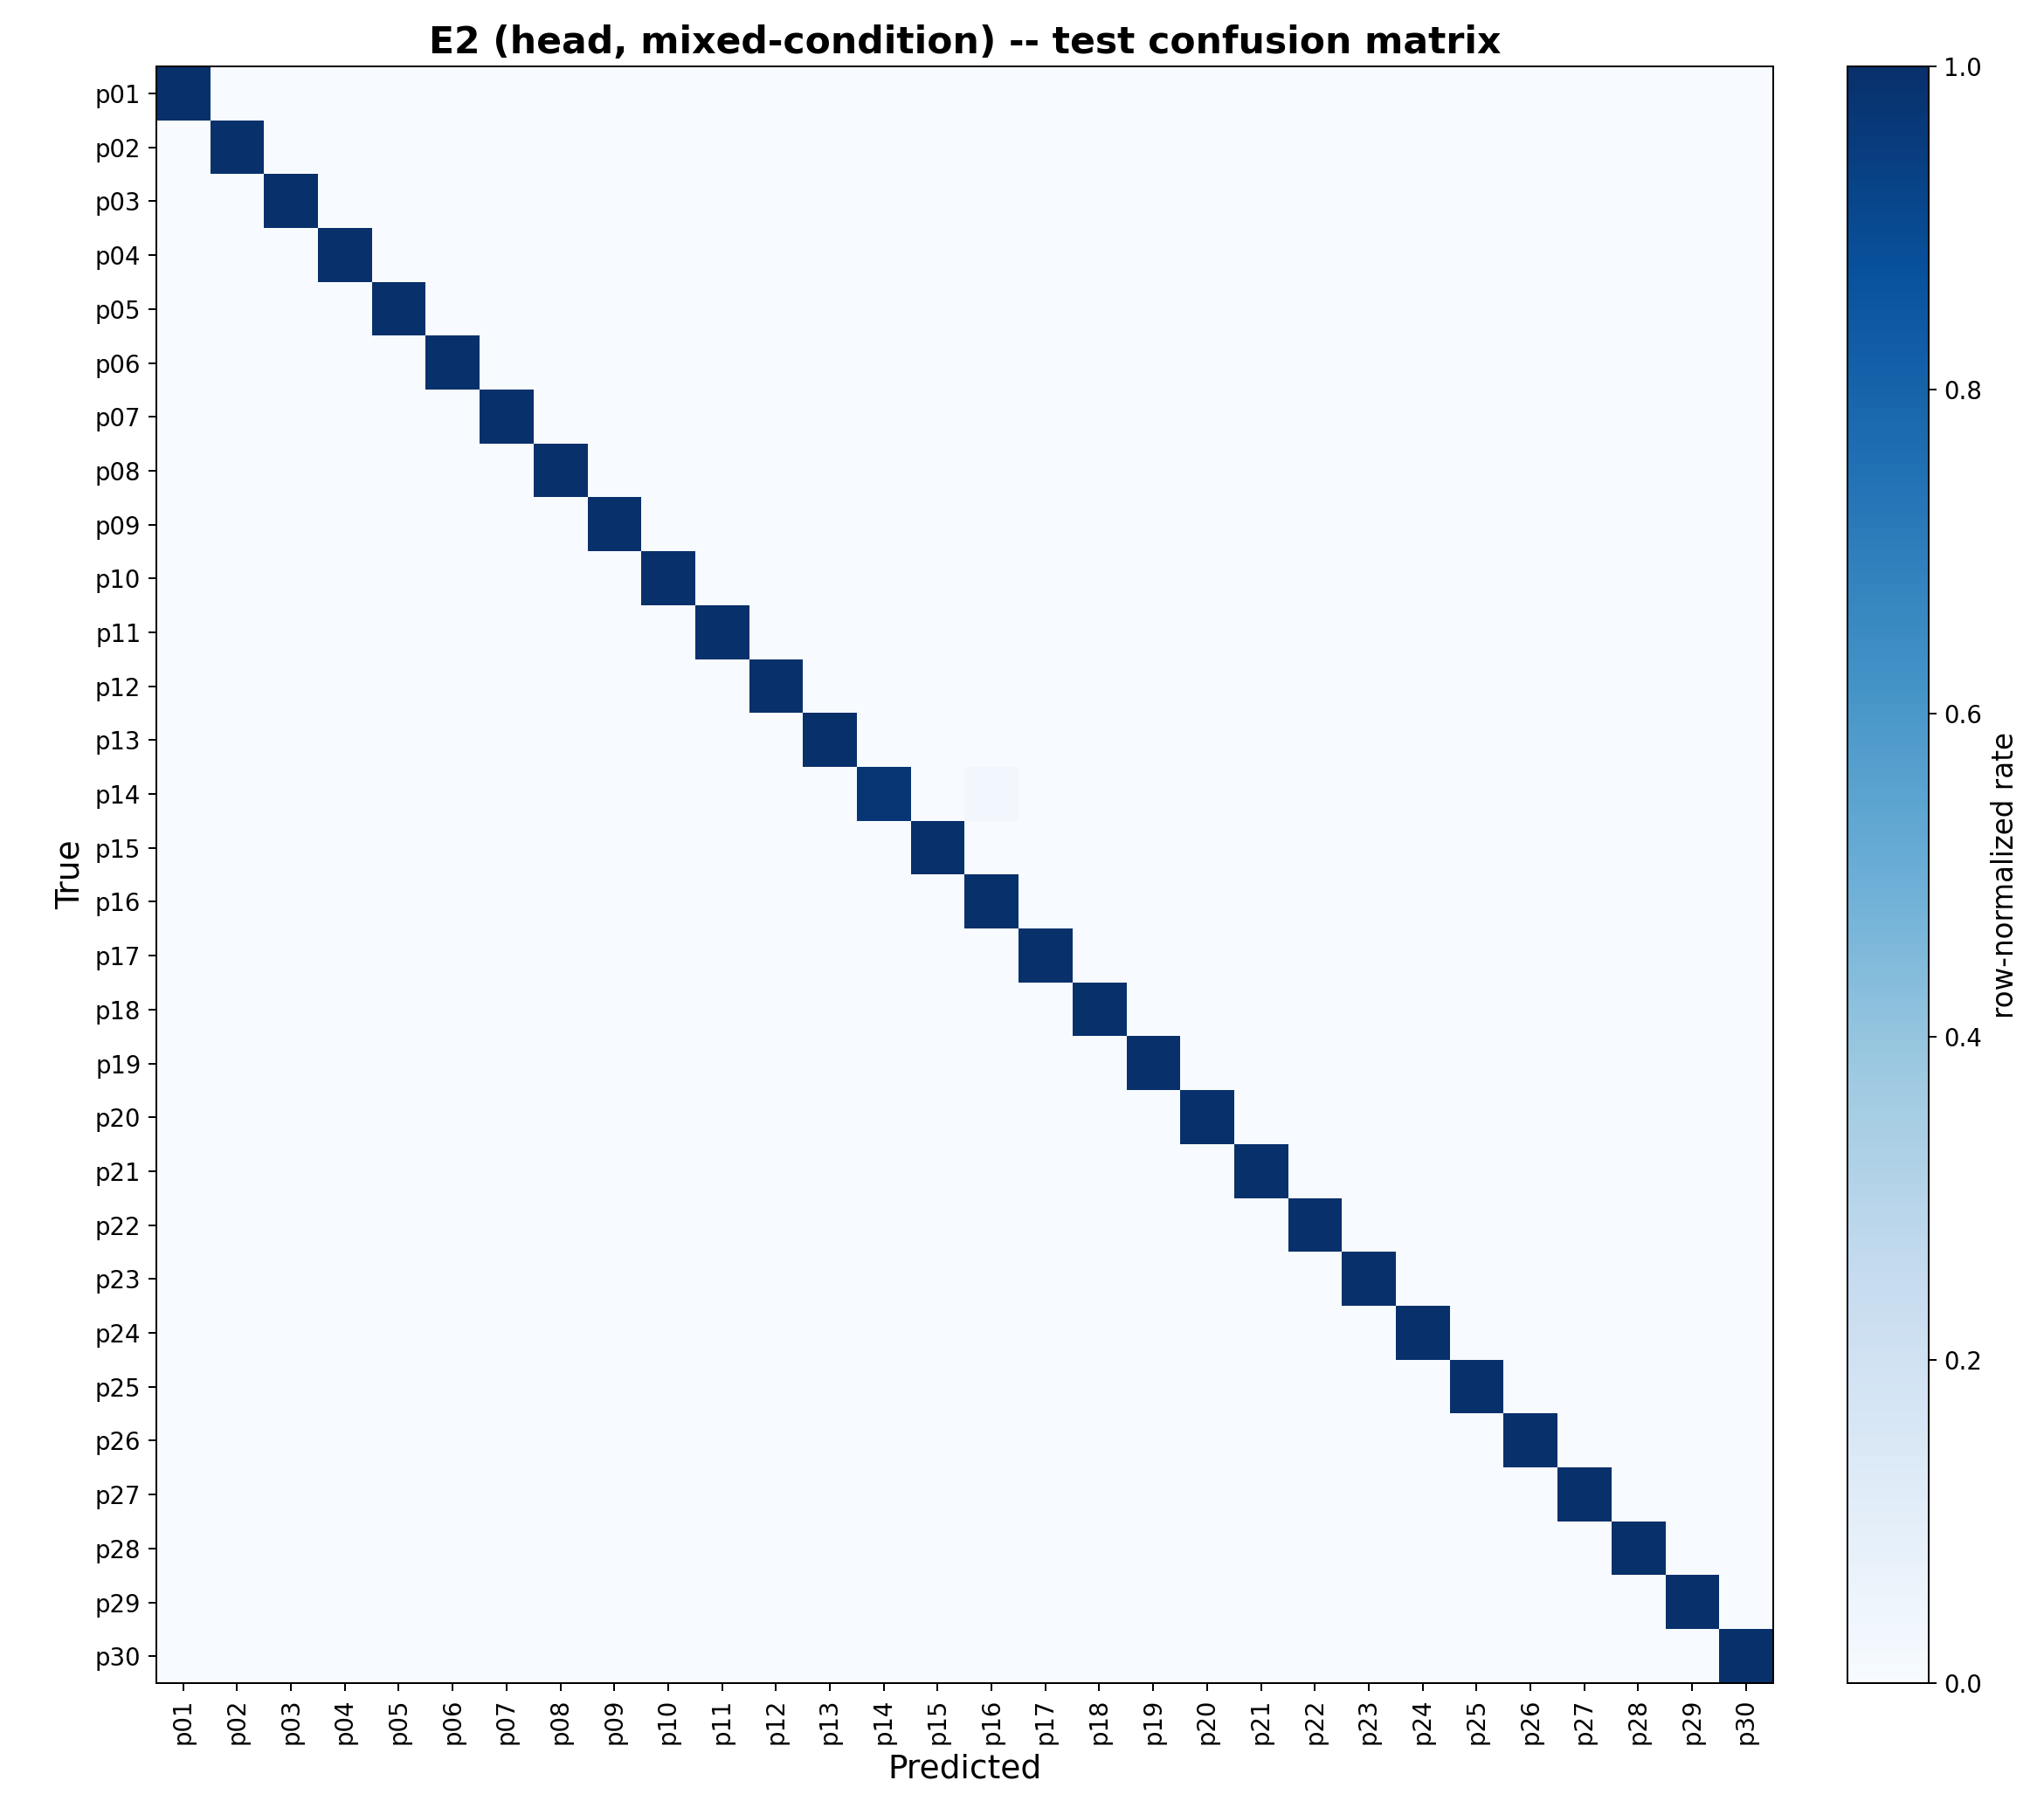
\includegraphics[width=0.92\linewidth]{figures/cm_large_e2.png}
\caption{Row-normalised $30\times30$ test confusion matrix, E2 (head, mixed-condition).}
\label{fig:confusion-e2}
\end{figure}

\section{Comparison with Related Work}
\label{sec:comparison}

Table~\ref{tab:comparison} places this project side by side, aspect by aspect, with its two base papers from Section~\ref{sec:related}: Pgu-Face, the closest dataset/capture precedent, and Chong et al., the closest recognition-method precedent. The comparison is necessarily approximate, since neither base paper evaluates the same task, scale, or identity pool as this project.

\begin{longtable}{L{2.6cm}L{3.6cm}L{3.9cm}L{4.1cm}}
\caption{Detailed three-way comparison: Pgu-Face (dataset base), Chong et al. (method base), and this project.}
\label{tab:comparison}\\
\toprule
\textbf{Aspect} & \textbf{Pgu-Face \cite{pguface2016}} & \textbf{Chong et al. \cite{chong2022svm}} & \textbf{This project} \\
\midrule
\endfirsthead
\toprule
\textbf{Aspect} & \textbf{Pgu-Face \cite{pguface2016}} & \textbf{Chong et al. \cite{chong2022svm}} & \textbf{This project} \\
\midrule
\endhead
Paper type & Dataset / Data in Brief article & Recognition method paper & Applied ML system \\
Primary objective & Create a partially-covered face dataset & Recognise masked faces using CNN + SVM & Identify known people under multiple real occlusions \\
Identities & 224 & RMFD 525 / LFW-SMFD 5{,}713 full; main experiments use 50 & 30 \\
Images & 896 & 90{,}000 (RMFD); 13{,}027 (LFW-SMFD); subsets used for experiments & 6{,}000 captured / 5{,}988 processed \\
Occlusion conditions & Sunglasses + facial-hair conditions & Primarily masks & Masks, sunglasses, clear glasses, scarves, caps, combinations \\
Capture source & Several consumer/mobile and commercial cameras & Public benchmark datasets & Local real capture (phone cameras) \\
Face detection & Not a proposed pipeline & Not central to the method & RetinaFace \\
Alignment & Not proposed as a recognition pipeline & Not central & Five-point landmark alignment \\
Feature representation & No proposed recognition representation & CNN feature vector & 512-D pretrained ArcFace embedding \\
Recognition model & None proposed & CNN + SVM & Pretrained ArcFace + 30-way local head \\
Training model & No recognition training model & CNN trained for feature extraction; SVM classifies labels & Head training; optional partial backbone fine-tuning \\
Training data strategy & Dataset construction & Masked + unmasked customised training & Clean-only vs.\ mixed-condition vs.\ partial fine-tuning \\
Epochs & Not applicable & 100, in reported experiments & Early stopping for E1/E2; fine-tuning for E3 \\
Best reported recognition result & Not applicable & 98.39\% TAR (RMFD, 50-category); 95.24\% TAR (LFW-SMFD, 50-category) & 99.90\% (E2); 100.00\% (E3) \\
Scalability & Dataset-oriented & Strong degradation as SVM category count grows & Not tested at large-scale / open-set \\
Deployment & None & Research evaluation only & Live phone-browser demo over HTTPS \\
Main value to this project & Dataset/capture precedent & Algorithmic/method precedent & Modern pretrained adaptation + broader occlusion + live deployment \\
\bottomrule
\end{longtable}

The key qualitative takeaway is not that this project "beats" either base paper — Pgu-Face proposes no recognition model to beat, and Chong et al.'s strongest number (98.39\% TAR) comes from a different dataset, a different evaluation protocol, and a 50-identity SVM setting that the same paper shows degrading sharply as more identities are added. This project's own strongest controlled comparison is E1 (94.29\%) to E2 (99.90\%) — a same-architecture, same-data-scale, occlusion-diversity-only change — which is a fair, apples-to-apples result in a way that any cross-paper accuracy comparison cannot be. The contribution here is not a new method, but a practical adaptation: a modern pretrained representation in place of a from-scratch CNN+SVM pipeline, a broader real occlusion set than either base paper covers, and a working live deployment neither base paper attempts.

\section{Deployment — Live Demonstration}
\label{sec:deployment}

\subsection{Model Selection and Live Switching}

The demo runs a dropdown that selects between E1, E2, and E3 live, without restarting the server — each request runs full detection, alignment, embedding, and classification for whichever experiment is currently selected. \textbf{E2 (head, mixed-condition) is the default}, since it is close to E3's accuracy (99.90\% vs.\ 100.00\%) without needing E3's heavier, CPU-converted backbone to be loaded first. A per-identity mean-embedding \emph{gallery} classifier with a calibrated \texttt{UNKNOWN}-rejection threshold (0.3179, from the 1st percentile of genuine train-centroid-vs-held-out-validation cosine-similarity scores) is implemented in the codebase (\texttt{scripts/07\_build\_gallery.py}) but is currently disabled in the demo dropdown; consequently, E1/E2/E3 are all closed-set only in the live demo as it stands — every detected face is assigned one of the 30 enrolled identities, with no mechanism yet active to flag an unenrolled visitor.

\subsection{Live Phone-Camera Demo}

The demo runs as a Flask web server on a laptop, serving a browser page to a phone over the local Wi-Fi network via HTTPS (a self-signed certificate, generated once and reused across restarts). The phone's camera streams frames to the server roughly every 400\,ms via \texttt{getUserMedia} (900\,ms when E3 is selected, since its converted backbone is heavier on CPU); each frame is detected, aligned with the identical \texttt{align\_crop} function used in preprocessing, embedded with whichever model is currently selected, averaged over a short rolling buffer of recent frames for temporal stability (cleared on every mode switch, since E3 uses a different embedding space from E1/E2), and classified. The result — participant name/ID and similarity score — is rendered back on the phone screen in real time. A device/camera-lens picker is included so the operator can choose a sharper physical camera on phones with multiple rear lenses (e.g.\ avoiding an ultra-wide lens), and a front/back camera toggle is provided. Figure~\ref{fig:demo-ui} shows the page's idle state, with the model dropdown, camera picker, and controls visible; Figure~\ref{fig:inference-pipeline} shows the full request pipeline this triggers on every frame.

\begin{figure}[htbp]
\centering
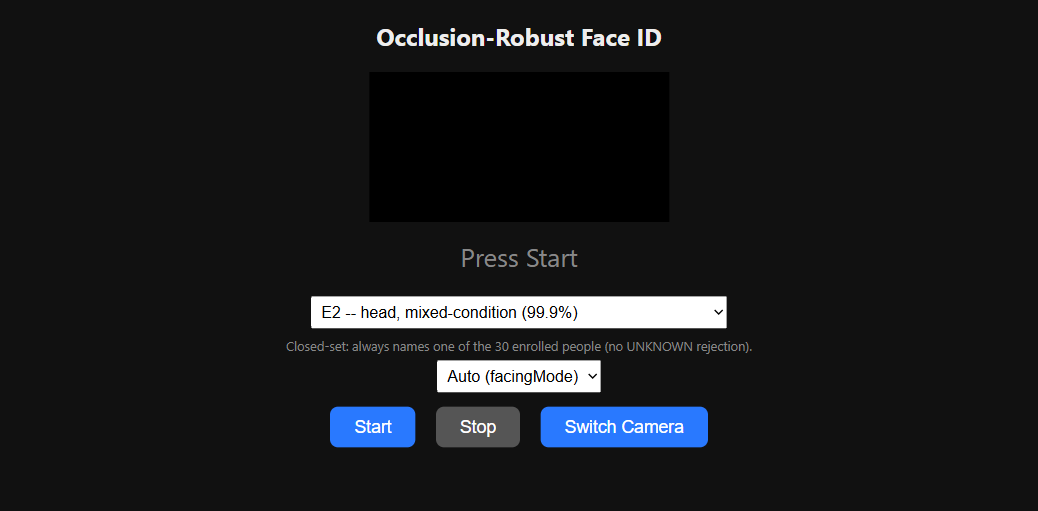
\includegraphics[width=0.55\linewidth]{figures/demo_app_ui.png}
\caption{The live demo's web interface (idle state, before the camera is started), captured directly from the running server.}
\label{fig:demo-ui}
\end{figure}

\begin{figure}[htbp]
\centering
\resizebox{\linewidth}{!}{%
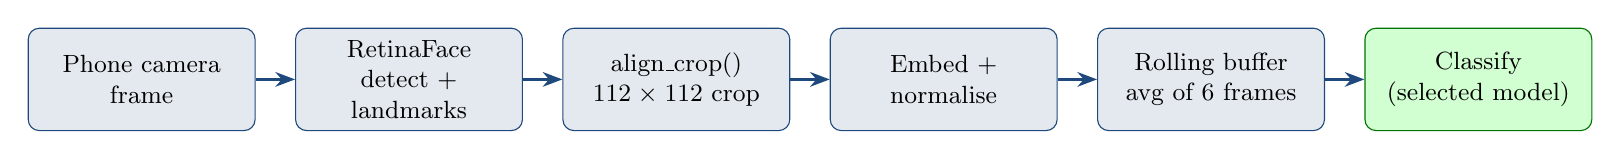
\begin{tikzpicture}[node distance=0.5cm]
\node[pbox] (photo) {Phone camera\\frame};
\node[pbox, right=of photo] (det) {RetinaFace\\detect + landmarks};
\node[pbox, right=of det] (align) {align\_crop()\\$112\times112$ crop};
\node[pbox, right=of align] (emb) {Embed +\\normalise};
\node[pbox, right=of emb] (buf) {Rolling buffer\\avg of 6 frames};
\node[pboxend, right=of buf] (cls) {Classify\\(selected model)};
\draw[parrow] (photo) -- (det);
\draw[parrow] (det) -- (align);
\draw[parrow] (align) -- (emb);
\draw[parrow] (emb) -- (buf);
\draw[parrow] (buf) -- (cls);
\end{tikzpicture}%
}
\caption{Live inference pipeline: what happens between one camera frame arriving at the server and a label being sent back to the phone.}
\label{fig:inference-pipeline}
\end{figure}

\section{Limitations and Future Work}
\label{sec:limitations}

\begin{itemize}
\item \textbf{Closed set only.} Every input is forced into one of 30 identities in the current demo configuration (E1/E2/E3, none of which reject an unenrolled face); a gallery-based classifier with a calibrated rejection threshold exists in the codebase but is currently disabled (Section~\ref{sec:deployment}). No formal open-set evaluation (e.g.\ measuring false-accept rate against genuinely unenrolled people) was performed either way.
\item \textbf{30 identities.} Results will not extrapolate to hundreds or thousands of enrolled people, and the closed-set numbers here are not comparable in absolute terms to the open-set, larger-scale results of Section~\ref{sec:comparison}.
\item \textbf{No anti-spoofing or liveness detection.} This is a laboratory classification prototype, not an access-control system, and would need a liveness check before any real deployment.
\item \textbf{Future work} suggested directly by Section~\ref{sec:related}'s base papers: an auxiliary mask-detection objective alongside identity, as in \cite{montero2022mtarcface}, or evaluating at a larger identity count to see whether the SVM-style scaling limits observed by \cite{chong2022svm} have any analogue here, could both be tested on a second, genuinely multi-session capture round.
\end{itemize}

\section{Supplementary Materials}
\label{sec:supplementary}

Beyond this report, the project repository includes three companion documents kept in sync with the code rather than restated here in full:

\begin{itemize}
\item \texttt{docs/arch.md} — four diagrams covering manual data curation, the constrained train/validation/test split, the training pipeline for E1--E3, and the inference pipeline as used by the live demo, each labelled with the actual repository file and folder names involved.
\item \texttt{docs/inference.md} — a step-by-step walkthrough of exactly what happens between a camera frame arriving and a label being returned, with a single worked example carried through every stage (detection output, aligned crop, raw and normalised embedding, classification).
\item \texttt{docs/models.md} — a one-table reference listing every model used in the project (RetinaFace, the frozen ArcFace backbone, the E1/E2 heads, the onnx2torch-converted E3 backbone), where each is used, and a one-sentence reason for its inclusion.
\end{itemize}

A 20-slide presentation summarising this report (\texttt{docs/presentation.pptx}) is also included, covering the same material with native, editable diagrams and the results charts reproduced in Section~\ref{sec:results}.

\section{Conclusion}

This project set out to build and evaluate a closed-set face-identification system robust to real occlusions, using a pretrained ArcFace model. Thirty participants were recruited and consented, and 6{,}000 images were collected across eight occlusion conditions and two lighting levels — well beyond the scale of Pgu-Face, the closest dataset precedent. A reproducible detect-align-crop pipeline processed 99.8\% of the dataset successfully, and a duplicate-aware, coverage-guaranteed split produced a 3{,}546/1{,}444/998 train/validation/test partition. Three experiments, evaluated with test accuracy and full confusion matrices, showed that training a classification head only on clean faces degrades specifically on the hardest combined occlusion, \texttt{mask+sunglasses} (E1, 94.29\% overall, 71.4\% on that condition), while training on occlusion-diverse data recovers full performance there and 99.90\% overall (E2); partial backbone fine-tuning closes the remaining gap entirely (E3, 100.00\%, perfect on every occlusion condition). The completed system was deployed as a live, phone-camera-driven demonstration accessible over the local network, defaulting to E2 with E1 and E3 selectable live via a dropdown. Compared against its two base papers, this project's pipeline is not offered as beating either — Pgu-Face proposes no recognition model, and Chong et al.'s CNN+SVM result comes from a different dataset and evaluation protocol entirely — but as a practical, modern adaptation: a pretrained ArcFace representation in place of a from-scratch CNN+SVM pipeline, a broader real occlusion set than either base paper covers, and a working live deployment neither attempts. The honest scientific contribution is the controlled, same-architecture E1-vs-E2 result: occlusion-diverse training data, not further architecture or loss engineering, is what closed the gap on the hardest occlusion condition.

\begin{thebibliography}{99}

\bibitem{deng2019arcface} J. Deng, J. Guo, N. Xue, and S. Zafeiriou, ``ArcFace: Additive Angular Margin Loss for Deep Face Recognition,'' in \emph{Proceedings of CVPR}, 2019.

\bibitem{deng2020retinaface} J. Deng, J. Guo, E. Ververas, I. Kotsia, and S. Zafeiriou, ``RetinaFace: Single-Shot Multi-Level Face Localisation in the Wild,'' in \emph{Proceedings of CVPR}, 2020.

\bibitem{pguface2016} S. R. Salari and H. Rostami, ``Pgu-Face: A Dataset of Partially Covered Facial Images,'' \emph{Data in Brief}, vol. 9, pp. 288--291, 2016. DOI: 10.1016/j.dib.2016.09.002.

\bibitem{chong2022svm} L. W. J. Chong, S.-C. Chong, and T.-S. Ong, ``Masked Face Recognition Using Support Vector Machine and Convolutional Neural Network,'' in \emph{Proceedings of the 10th International Conference on Information and Communication Technology (ICoICT)}, 2022, pp. 270--274. DOI: 10.1109/ICoICT55009.2022.9914874.

\bibitem{montero2022mtarcface} D. Montero, M. Nieto, P. Leskovsky, and N. Aginako, ``Boosting Masked Face Recognition with Multi-Task ArcFace,'' in \emph{Proceedings of SITIS}, 2022, pp. 184--189. DOI: 10.1109/SITIS57111.2022.00042.

\end{thebibliography}

\end{document}
